\section{Environment plug-in}

\subsection{Features}

\subsubsection{Mountains}

Our first implementation of the Mountain feature corresponded to what is presented in \cite{FeatureTree}. However, the 2D random functions we tried did not yield satisfying results. That's why we switched to another version, where we import at random a part of a heightmap taken from a website \cite{terrain-party}. This website import the heightmaps through satellite imaging.

\subsection{Graphical User Interface (GUI)}

A picture of the interface is presented in Fig.~\ref{fig:env-gui1}. Using the interface, the user can choose the feature he wants to draw. He can then draw it using a pencil integrated in Blender, drawing polygons here. After having completed the drawing of the features, the user can ask for the generation of the environment. It can then hide the polygons, and also modify parameters that are feature-specific.

\begin{figure}
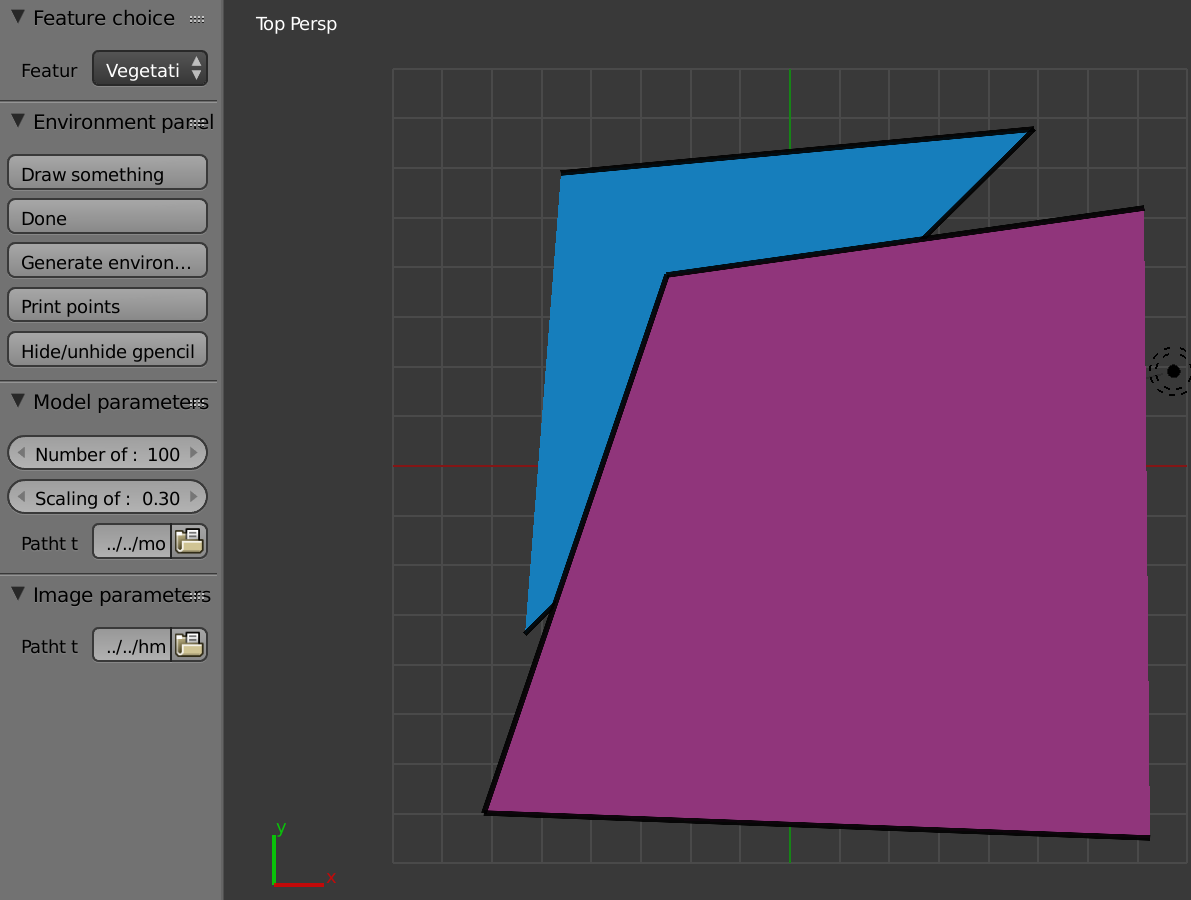
\includegraphics[width=\textwidth]{img/env_gui1.png}
\caption{GUI of the Environment plug-in, with two features (in blue and magenta)}
\label{fig:env-gui1}
\end{figure}

